\chapter{Конструкторский раздел}

В данном разделе описаны структура разрабатываемого ПО, используемые структуры данных, а также приведены схемы алгоритмов используемых при отрисовке изображения.

В данном разделе описаны требования, которым должно удовлетворять ПО, структура разрабатываемого ПО, используемые структуры данных, а также приведены схемы алгоритмов используемых при отрисовке изображения.

\section{Требования к ПО}

Создаваемое ПО должно предоставлять следующий функционал:

\begin{itemize}
	\item загрузка заготовленных полигональных моделей из файлов;
	\item добавление в сцену объектов из заготовленного набора примитивов;
	\item независимое трансформирование положения объектов в сцене;
	\item навигация по сцене с помощью перемещения и поворота главной камеры;
	\item просмотр и изменение специфических свойств объектов в сцене;
	\item сохранение текущего изображения сцены в файл на диске;
	\item сохранение созданной сцены в файл на диске;
	\item загрузка готовой сцены из файла.
\end{itemize}

\clearpage

\section{Структура ПО}

\subsection{Схема доменов}

Программное обеспечение будет состоять из трех доменов: прикладного, архитектурного и
интерфейсного. Прикладной домен будет отвечать за процесс визуализации сцены,
интерфейсный - за взаимодействие с пользователем, а архитектурный послужит связующим звеном между двумя вышеупомянутыми доменами.

На рисунке \ref{schema:domen} представлена схема доменов.

\begin{figure}[h]
	\centering
	
\includegraphics[width=\linewidth,height=0.85\textheight,keepaspectratio]{diagrams/domens.pdf}
	\caption{Схема доменов}
	\label{schema:domen}
\end{figure}

\subsection{Прикладной домен}

Для прикладного домена были подготовлены информационная модель и схема иерархии по данным.

\begin{figure}[h]
	\centering
	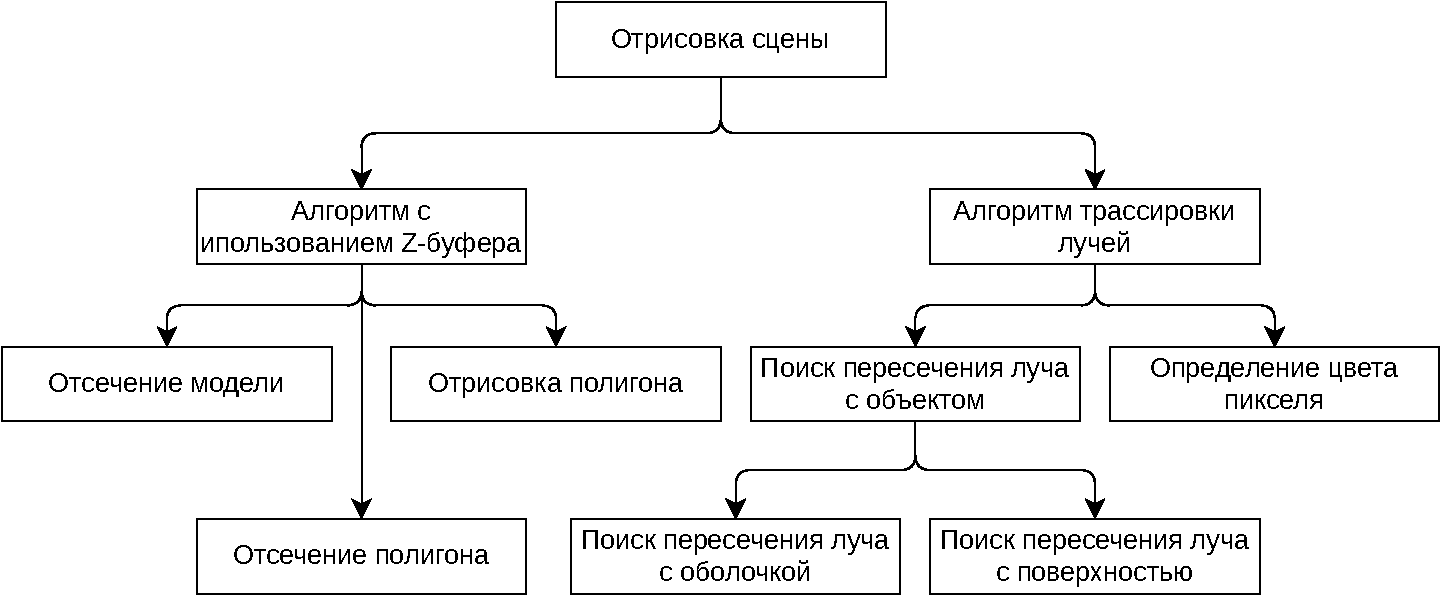
\includegraphics[width=\linewidth,height=0.85\textheight,keepaspectratio]{diagrams/core-info.pdf}
	\caption{Информационная модель прикладного домена}
\end{figure}

\begin{figure}[h]
	\centering
	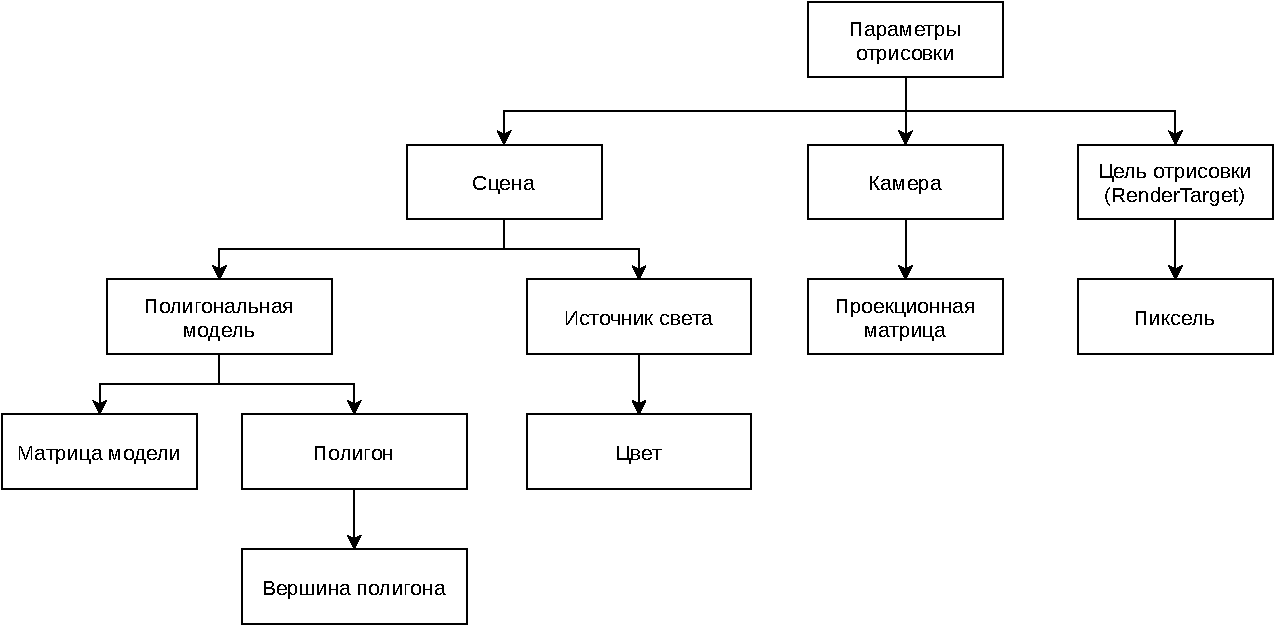
\includegraphics[width=\linewidth,height=0.85\textheight,keepaspectratio]{diagrams/core-data.pdf}
	\caption{Иерархия прикладного домена по данным}
\end{figure}

\clearpage

\subsection{Архитектурный домен}

Ниже на рисунке \ref{uml:arch} приведена иерархия классов для архитектурного домена.

\begin{figure}
	\centering
	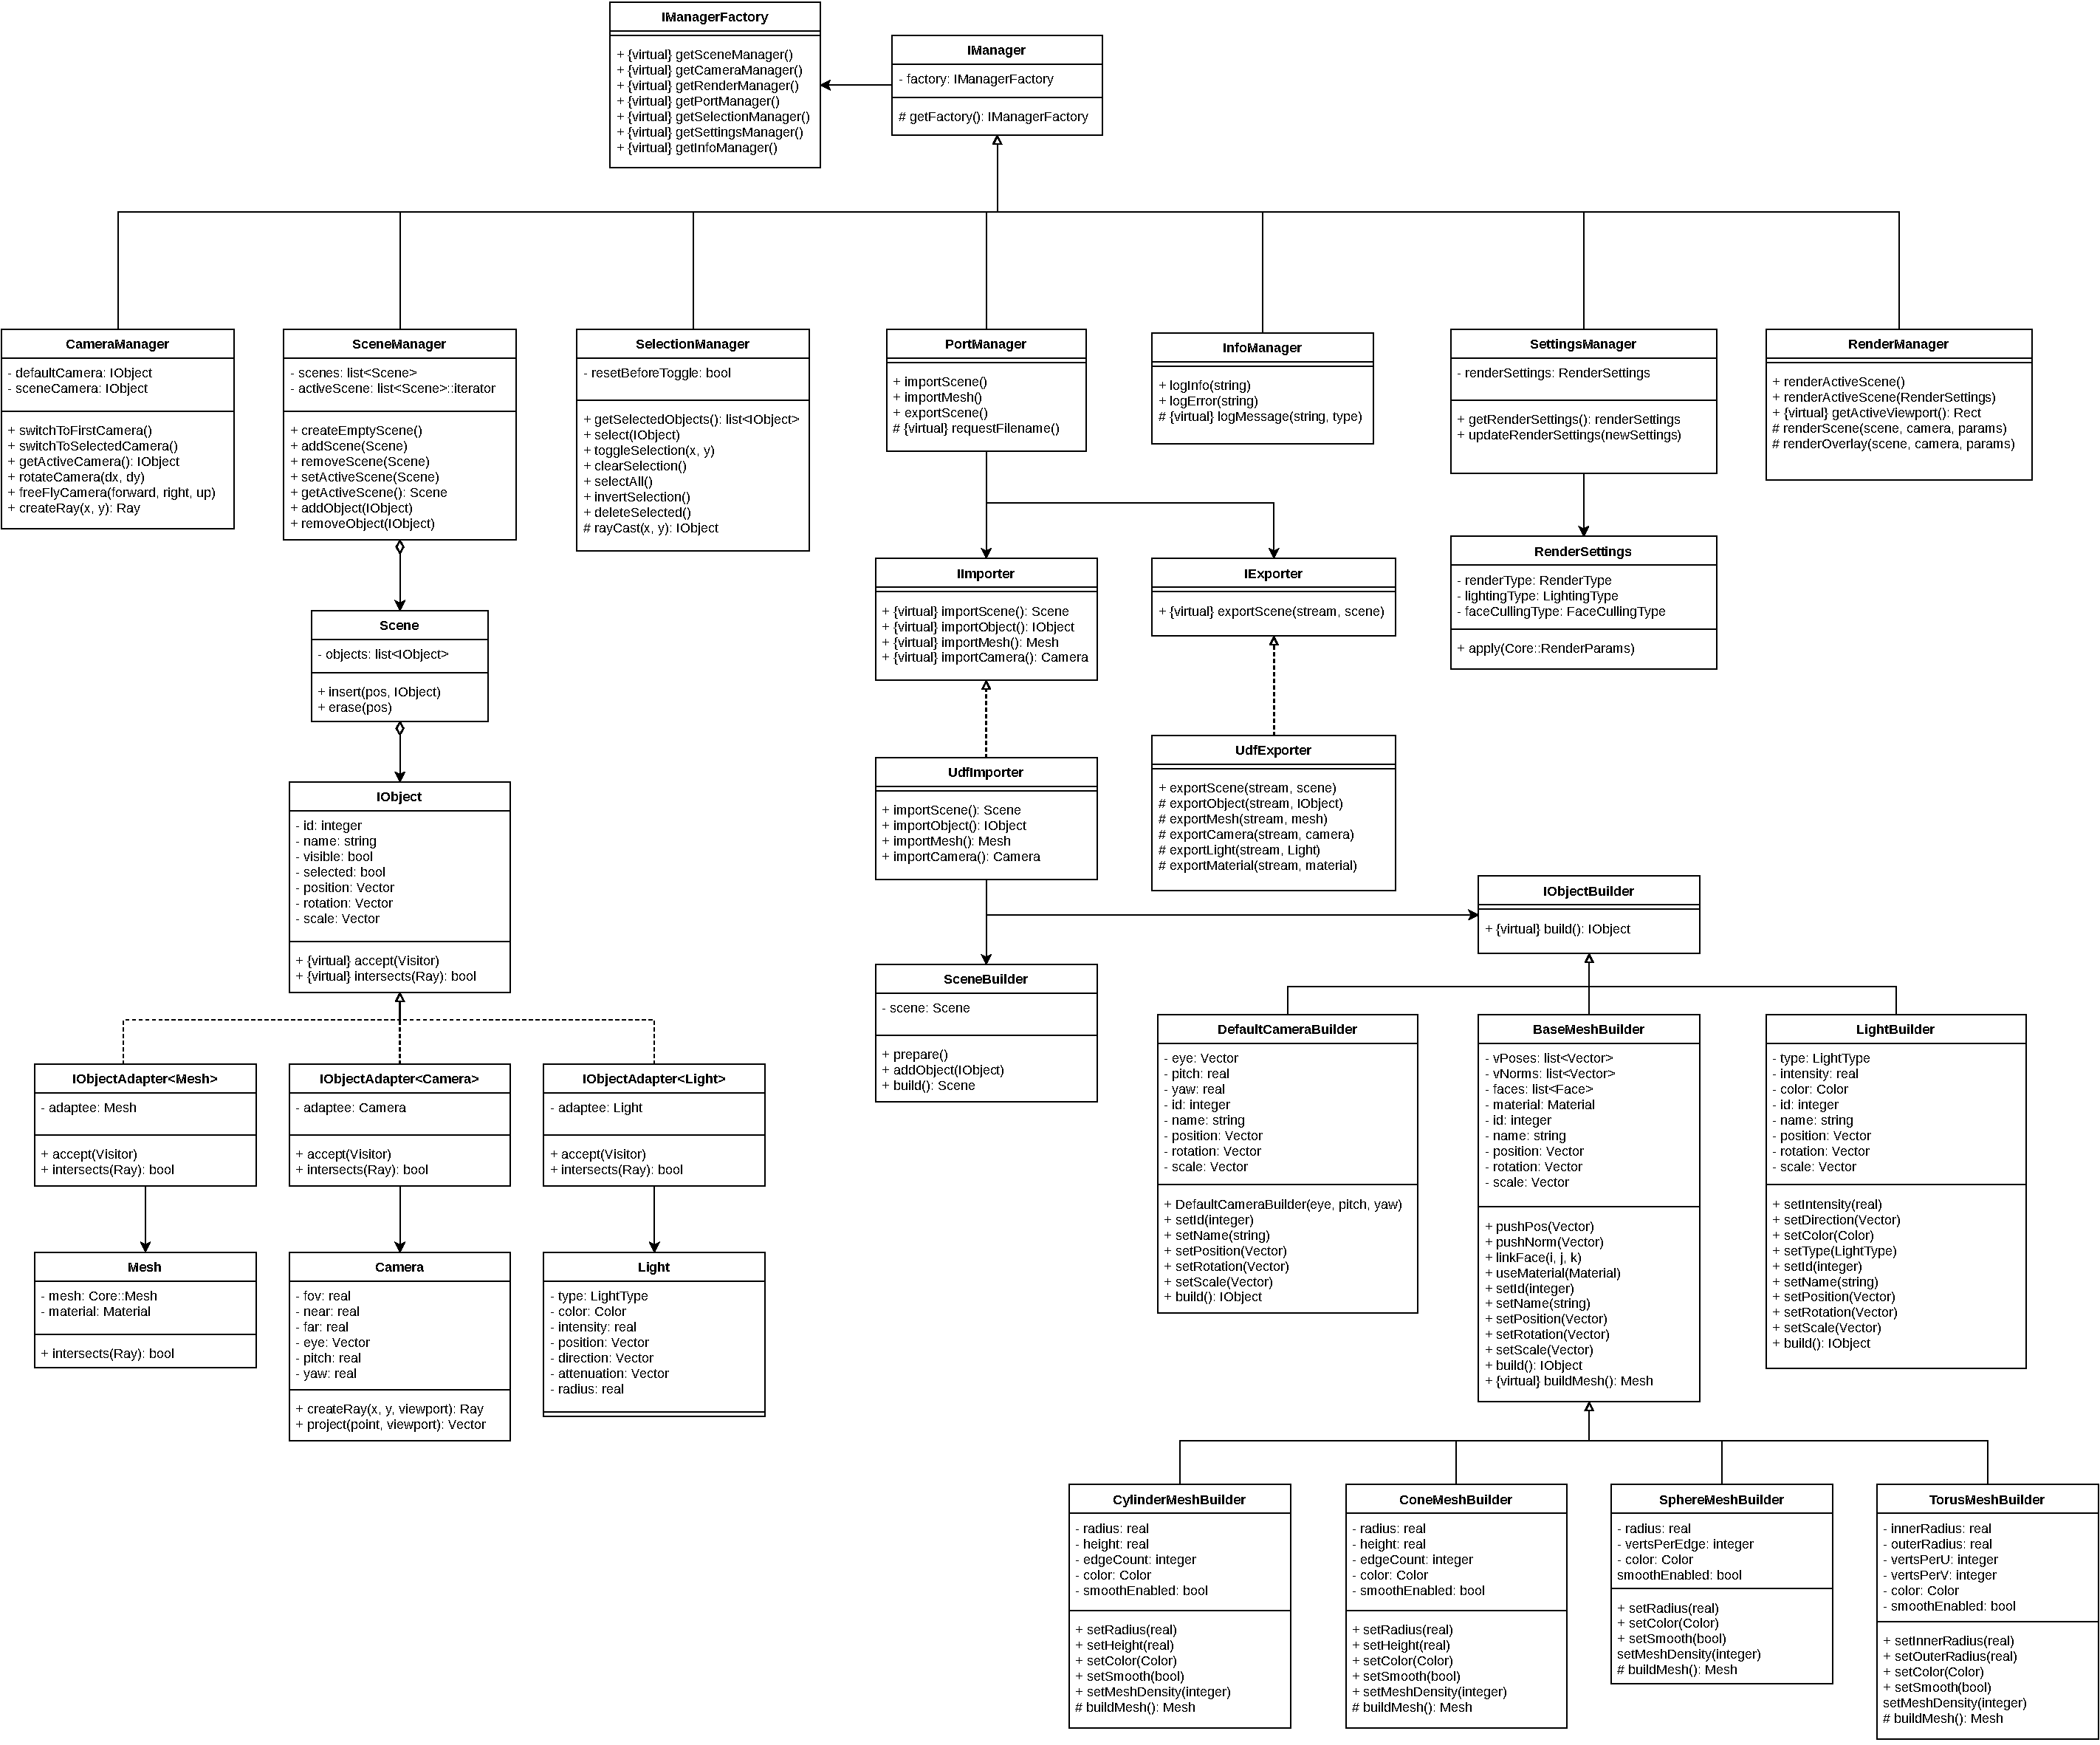
\includegraphics[angle=90,origin=c,width=\linewidth,height=0.85\textheight,keepaspectratio]{diagrams/uml.pdf}
	\caption{UML диаграмма классов архитектурного домена}
	\label{uml:arch}
\end{figure}

\clearpage

\subsection{Процесс синтеза изображения}

Ниже на рисунках \ref{idef0:render:1}--\ref{idef0:render:4} представлена IDEF0 диаграмма процесса синтеза изображения сцены.

\begin{figure}[ht]
    \centering
    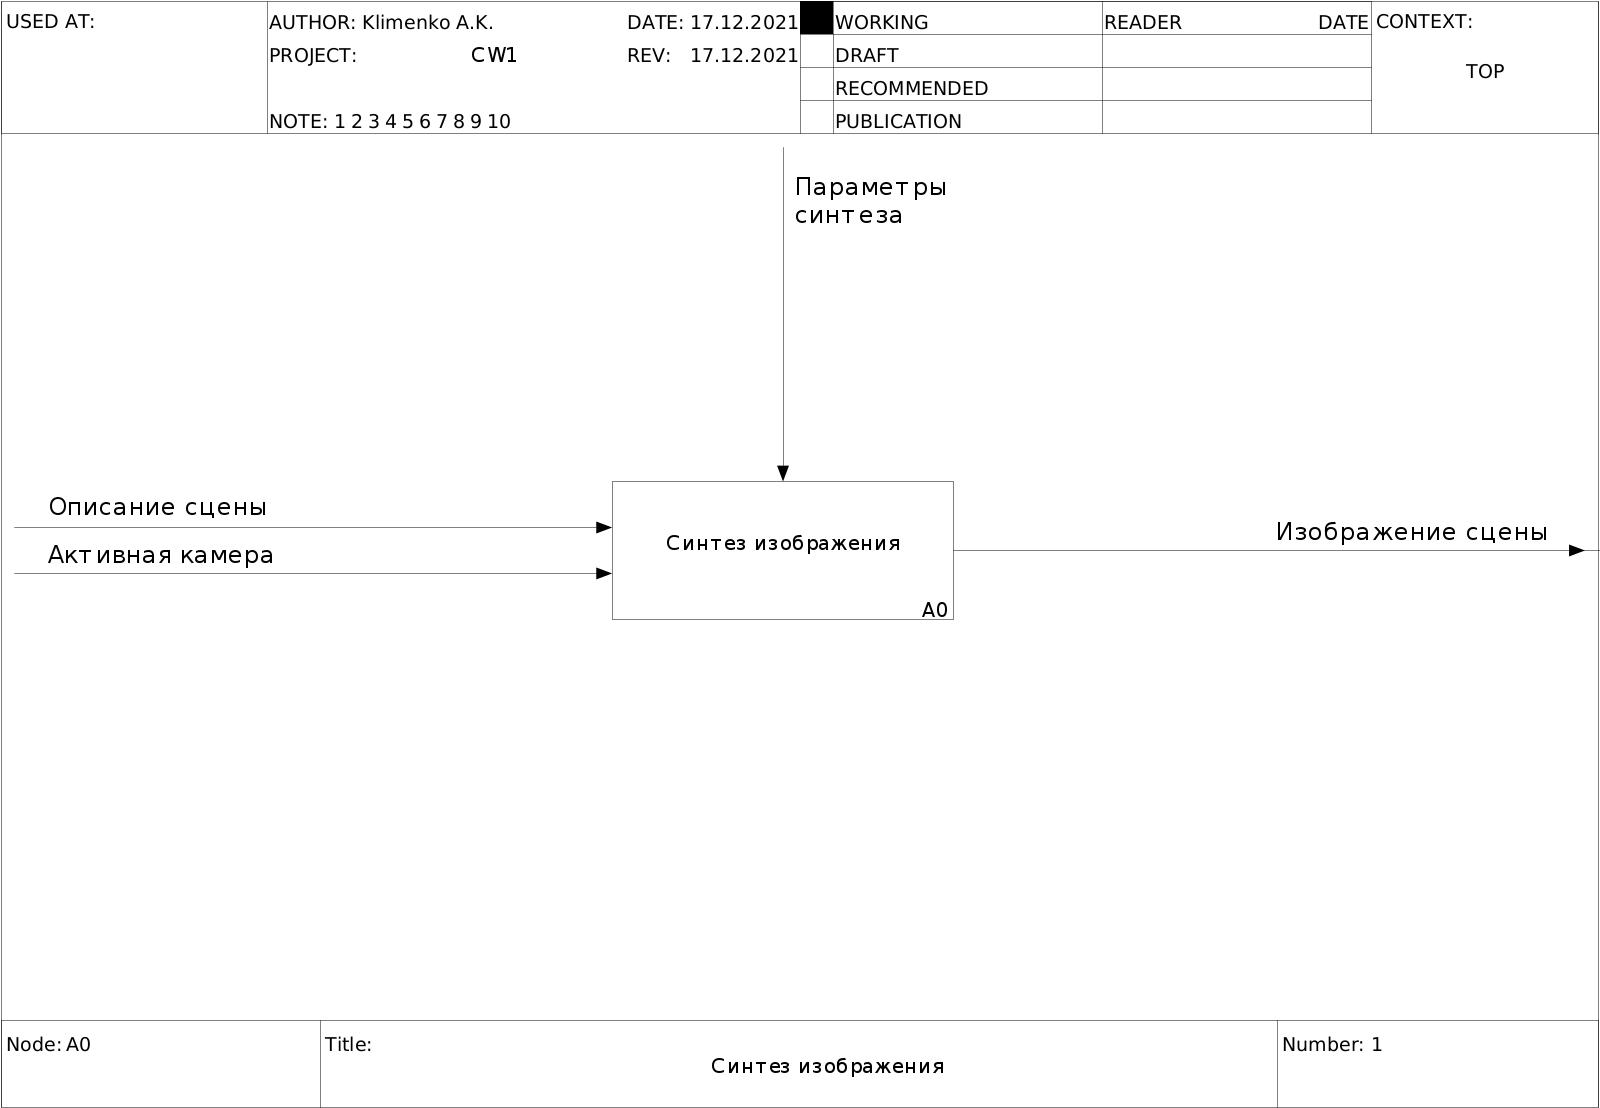
\includegraphics[width=\linewidth,height=0.85\textheight,keepaspectratio]{idef0/01_A0.jpg}
    \caption{IDEF0 диаграмма процесса синтеза изображения (часть 1)}
    \label{idef0:render:1}
\end{figure}

\begin{figure}
    \centering
    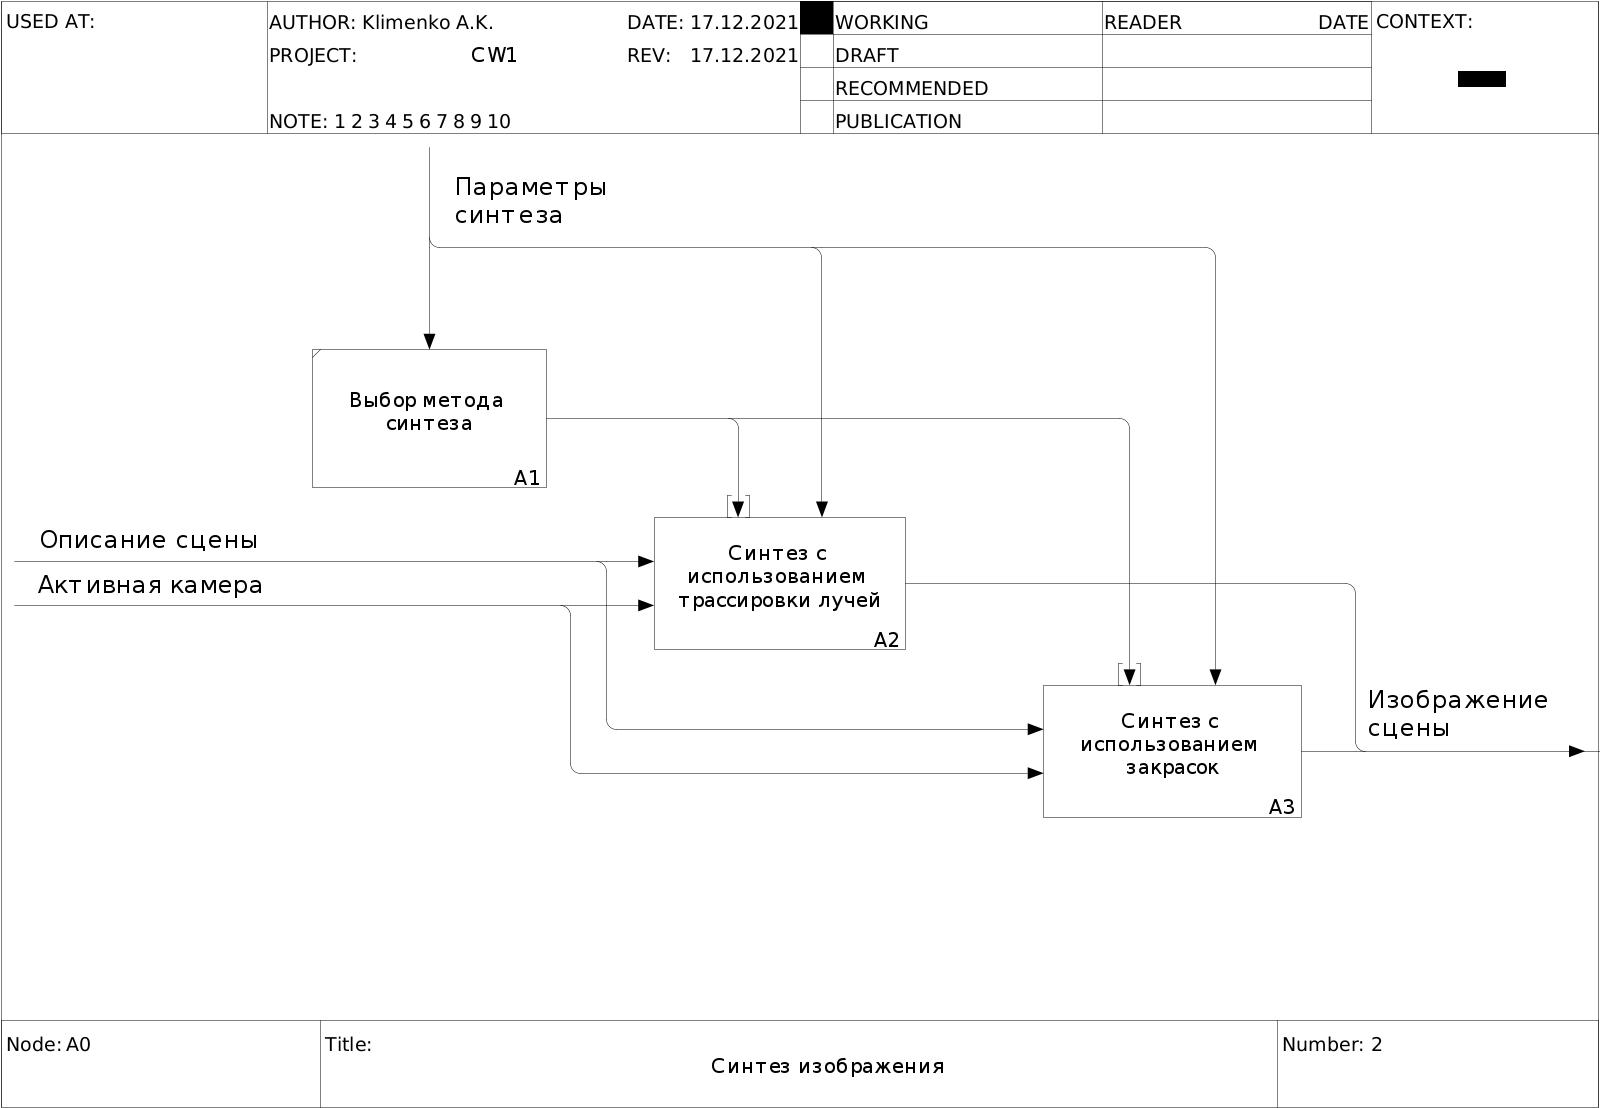
\includegraphics[width=\linewidth,height=0.85\textheight,keepaspectratio]{idef0/02_A0.jpg}
    \caption{IDEF0 диаграмма процесса синтеза изображения (часть 2)}
    \label{idef0:render:2}
\end{figure}

\begin{figure}
    \centering
    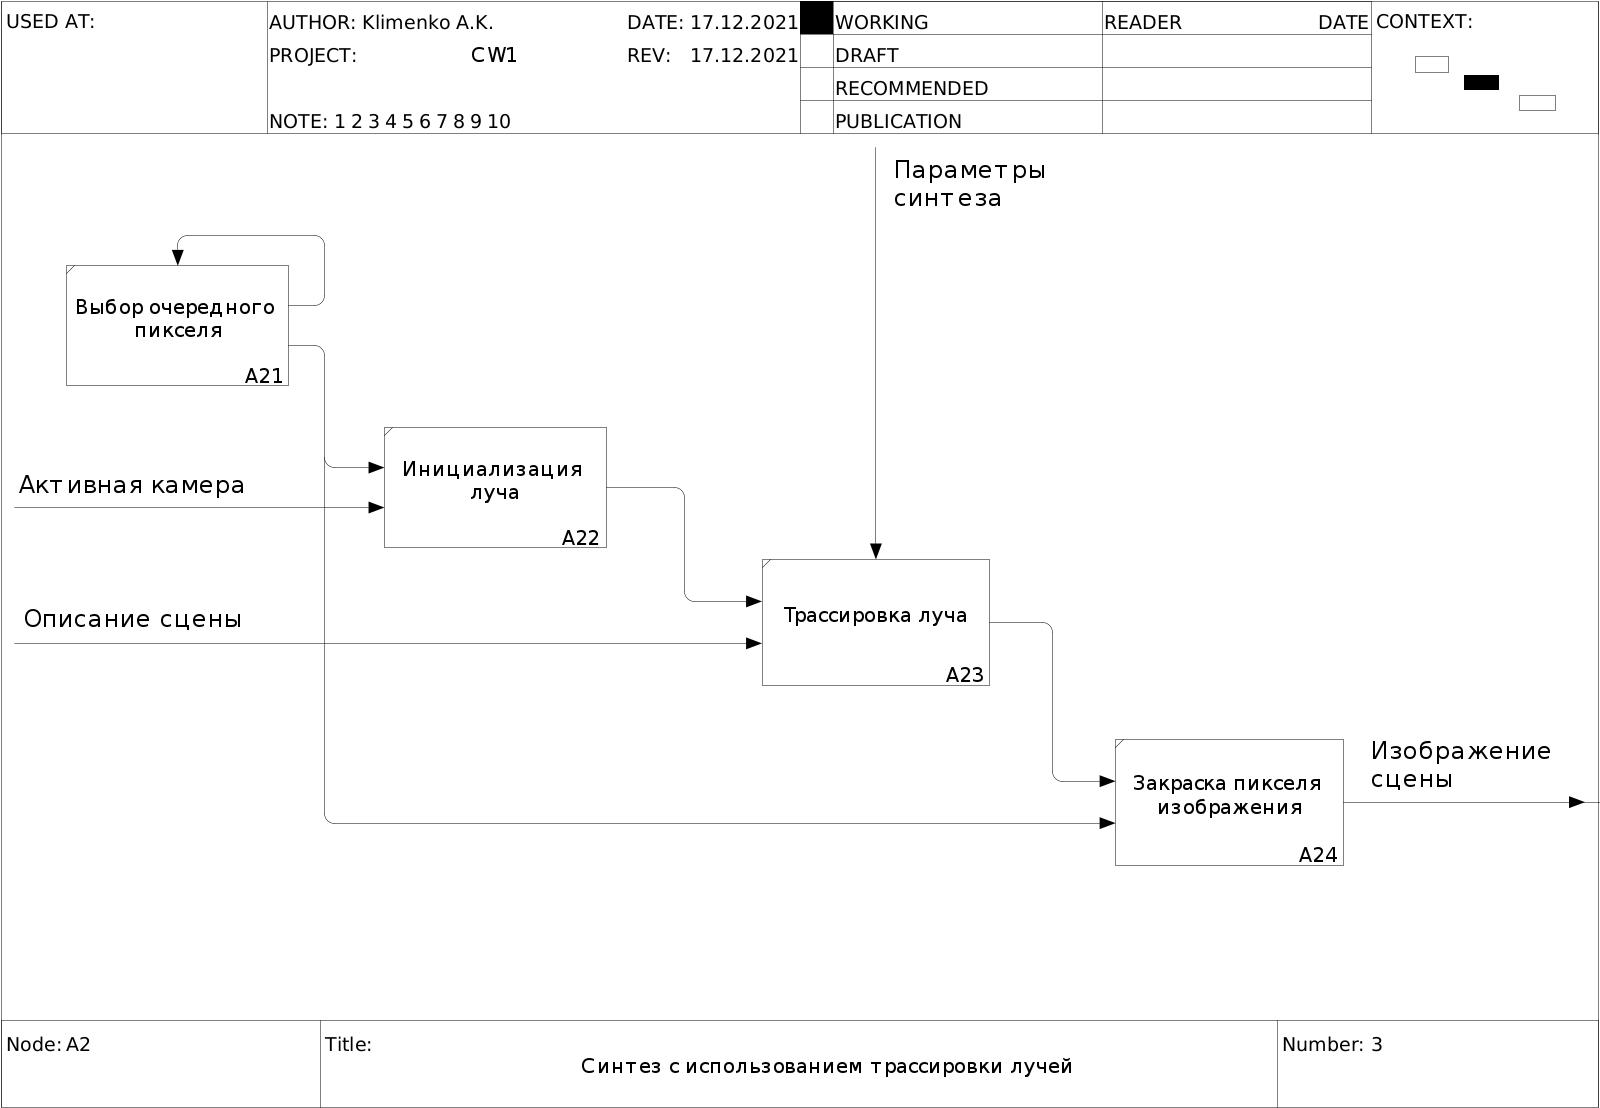
\includegraphics[width=\linewidth,height=0.85\textheight,keepaspectratio]{idef0/03_A2.jpg}
    \caption{IDEF0 диаграмма процесса синтеза изображения (часть 3)}
    \label{idef0:render:3}
\end{figure}

\begin{figure}
    \centering
    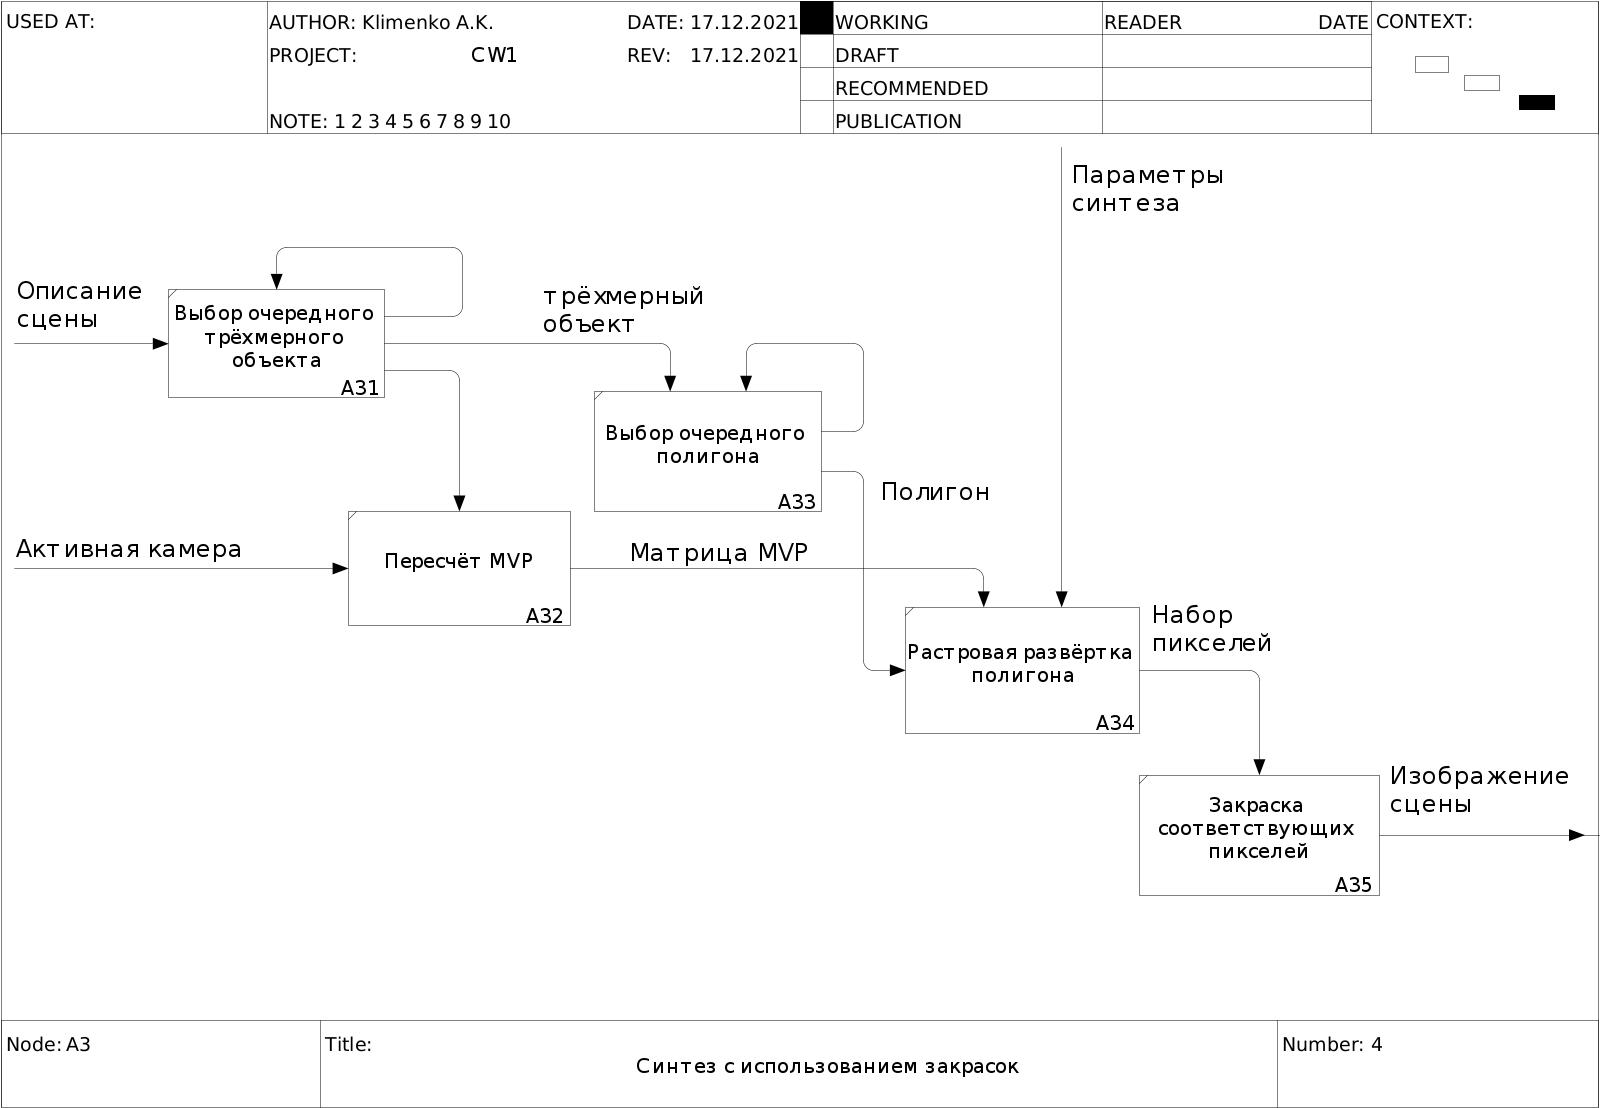
\includegraphics[width=\linewidth,height=0.85\textheight,keepaspectratio]{idef0/04_A3.jpg}
    \caption{IDEF0 диаграмма процесса синтеза изображения (часть 4)}
    \label{idef0:render:4}
\end{figure}

\clearpage

\section{Схемы алгоритмов}

В данной секции представлены 2 алгоритма синтеза изображения. Первый использует закраски полигонов, а второй -- метод трассировки лучей.

\subsection{Быстрая отрисовка}

На рисунках \ref{alg:fast:1}--\ref{alg:fast:2} представлен алгоритм синтеза изображения, использующий простые закраски.

\begin{figure}
	\centering
	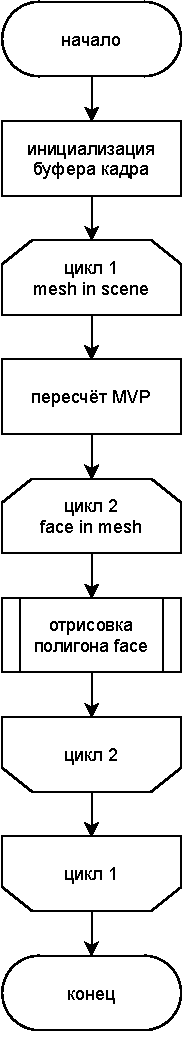
\includegraphics[width=\linewidth,height=0.85\textheight,keepaspectratio]{diagrams/fast.pdf}
	\caption{Алгоритм использующий простую закраску (часть 1)}
	\label{alg:fast:1}
\end{figure}

\begin{figure}
	\centering
	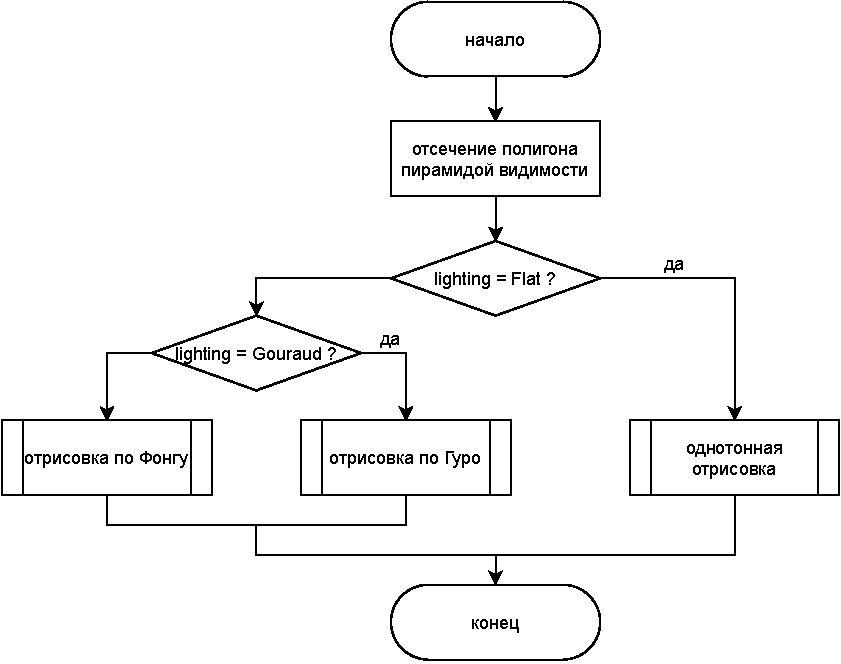
\includegraphics[width=\linewidth,height=0.85\textheight,keepaspectratio]{diagrams/draw-face.pdf}
	\caption{Алгоритм использующий простую закраску (часть 2)}
	\label{alg:fast:2}
\end{figure}

\clearpage

\subsection{Реалистичная отрисовка}

На рисунке \ref{alg:fancy} представлена схема алгоритма трассировки лучей.

\begin{figure}[h]
	\centering
	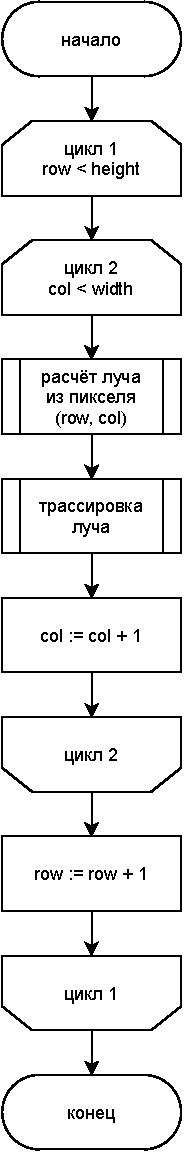
\includegraphics[width=\linewidth,height=0.7\textheight,keepaspectratio]{diagrams/fancy.pdf}
	\caption{Алгоритм использующий трассировку лучей}
	\label{alg:fancy}
\end{figure}

\clearpage

\section{Структуры данных}

В данной подсекции описываются основные структуры данных, необходмые для решения задачи синтеза изображения.

\subsection{Сцена}

В рассматриваемой задаче синтеза изображения сцена является элементом самого верхнего уровня, в полной мере содержащим информацию об объектах, находящихся на сцене, а также информацию об используемом освещении.

Данная структура данных будет использоваться прежде всего для отображения объектов, поэтому основным требованием, предъявляемым к ней, будет эфективная выборка объектов сцены. Из этого можно заключить, что наиболее выгодным с точки зрения производительности будет выбор массива в качестве контейнера для объектов сцены и источников освещения.

\subsection{Трёхмерное тело}

Рассматривая задачу синтеза изображения, любое трёхмерный объект можно разложить на две составляющие -- форму тела (его геометрию), и оптические свойства поверхности материала, из которого изготовлен объект.

Выбор структуры трёхмерного тела должен выполняться в соответствии с выбранными алгоритмами решения поставленной задачи. В следствии чего было принято решение об использовании массива треугольников в качестве описания геометрии объекта.

Оптические свойства поверхности объекта будут описаны в отдельной структуре -- материал. Она будет включать в себя такие параметры, как: цвет фонового освещения, цвет направленного освещения, цвет бликов. Также данная структура будет содержать следующие параметры для синтеза реалистичного изображения: коэффициенты прозрачности, отражния и преломления, а также показатель преломления среды.

\subsection{Источник освещения}

В постановке задачи синтеза изображения выделены следующие типы источников освещения: фоновый, направленный и точечный. Далее каждый тип будет рассмотрен в отдельности.

\textbf{Фоновое освещение.} Фоновая освещённость объектов в сцене не зависит от положения источника света в пространстве, а зависит только от цвета освещения и его интенсивности.

\textbf{Направленное освещение.} Для данного типа освещения необходимо хранить его цвет, интенсивность и направление.

\textbf{Точечное освещение.} Данный тип освещения регулируется положением источника в пространстве, радиусом освещения и коэффициентами затухания.

%\section{Тестирование ПО}
